\section{Implementation Details about \textsc{RATs}}
\label{sec:appendix_agent_team}
This section provides implementation details for \textsc{RATs}
introduced in Sec.~\ref{sec:method}. 
We introduce the details of the three teams that make up \textsc{RATs}: the \emph{Task Proposer} team (play-time task proposal), the \emph{Execution} team (task execution), and the \emph{Memory-Management} team (skill library and failure memory updates).
We then describe how the learned skill
library is used during evaluation and summarize the prompt interfaces of each
agent.


\subsection{Details of Play-Time Task Proposal}
\label{sec:appendix_task_proposal}

\textbf{Candidate task generation.}
At each play iteration, the Task Proposer receives the current scene context, a
compact summary of the skill library $\mathcal{L}$, and a short history of
recent attempts. The skill summary includes each learned skill's name,
description, reliability tier, and empirical success statistics, but not its
full source code. This lets the proposer reason about available capabilities
and explored object-skill pairs without filling the context with code. The
proposer then generates a candidate pool $\mathcal{T}_t$ of play tasks, along
with the objects and skills required by each candidate.

The scene context is instantiated differently across environments. In LIBERO,
the proposer uses the object inventory and available manipulation primitives.
In MolmoSpaces, object identifiers are first grounded into readable phrases
from the current visual observation, and only visible, reachable objects are
shown as proposal targets. This prevents the proposer from selecting objects
that exist in the scene metadata but are not accessible from the robot's
current state.

\textbf{Goldilocks-driven task selection.}
After candidate generation, we score each candidate using the Goldilocks
objective in Sec.~\ref{sec:proposer}. The novelty term is computed from
historical counts over object-skill pairs. The competence estimate uses the
Wilson lower bound of each required skill's empirical success rate, rather than
the raw success rate, so that a rarely used skill is not treated as reliable
after one lucky success. We rank candidates by the product of object-skill
novelty and competence-frontier score. We also downweight tasks that closely
match recent failures. Diagnosable failures with initially plausible plans are
stored in a bounded retry bank, which can later propose simplified variants
with a decaying retry bonus.

\textbf{Environment creation.}
After a task is selected, the Environment Creator converts the proposal into an
executable task instance. In LIBERO, it generates a BDDL task specification,
validates its syntax and semantics, and instantiates the corresponding MuJoCo
environment. Static checks require all referenced objects, fixtures, regions,
predicates, and assets to match the proposal. If validation fails, the creator
performs one bounded repair and validates the repaired specification again. A
compact example is shown below.

\begin{verbatim}
(:language pick up the butter and put it on the plate)
(:objects butter_1 - butter plate_1 - plate)
(:init
  (On butter_1 kitchen_table_butter_init_region)
  (On plate_1 kitchen_table_plate_init_region))
(:goal (And (On butter_1 plate_1)))
\end{verbatim}

\textbf{Environment verification.}
Before a LIBERO task enters the execution stage, the Environment Verifier runs
deterministic checks over two reset seeds. The environment must instantiate and
render successfully, expose the simulator, realize each declared object body,
evaluate every goal predicate without error, and avoid severe initial
penetrations. In MolmoSpaces, task creation is constrained by the bridge
catalog. After rebinding the environment, the verifier checks that the proposed
target remains visually grounded. Rejected tasks return to the task proposing stage
rather than consuming an execution attempt.

\subsubsection{Example Trace of Play-Time Task Proposal}
Table~\ref{tab:proposal_selection_example} and Figure~\ref{fig:play_task_proposal} show the saved candidate trace from
MolmoSpaces play iteration 15. Scene grounding first marks five objects as
visible: a blue spray bottle, black cloth, brown tissue box, toilet, and white
cabinet. Reachability filtering removes the toilet, leaving four usable
main targets for proposal. The Task Proposer receives these targets together
with the exact current library of 22 skills (13 primitives and 9 learned
skills) and the previous 10 task records, then generates $K=5$ candidates. The
selected tissue-box lift receives the highest composite score ($0.6236$): it is
novel but remains close enough to the robot's current grasping capabilities to
be worth practicing. The black-cloth pick is vetoed before ranking because its
interaction is unsupported in the active bridge configuration.

\begin{figure}[t]
\centering
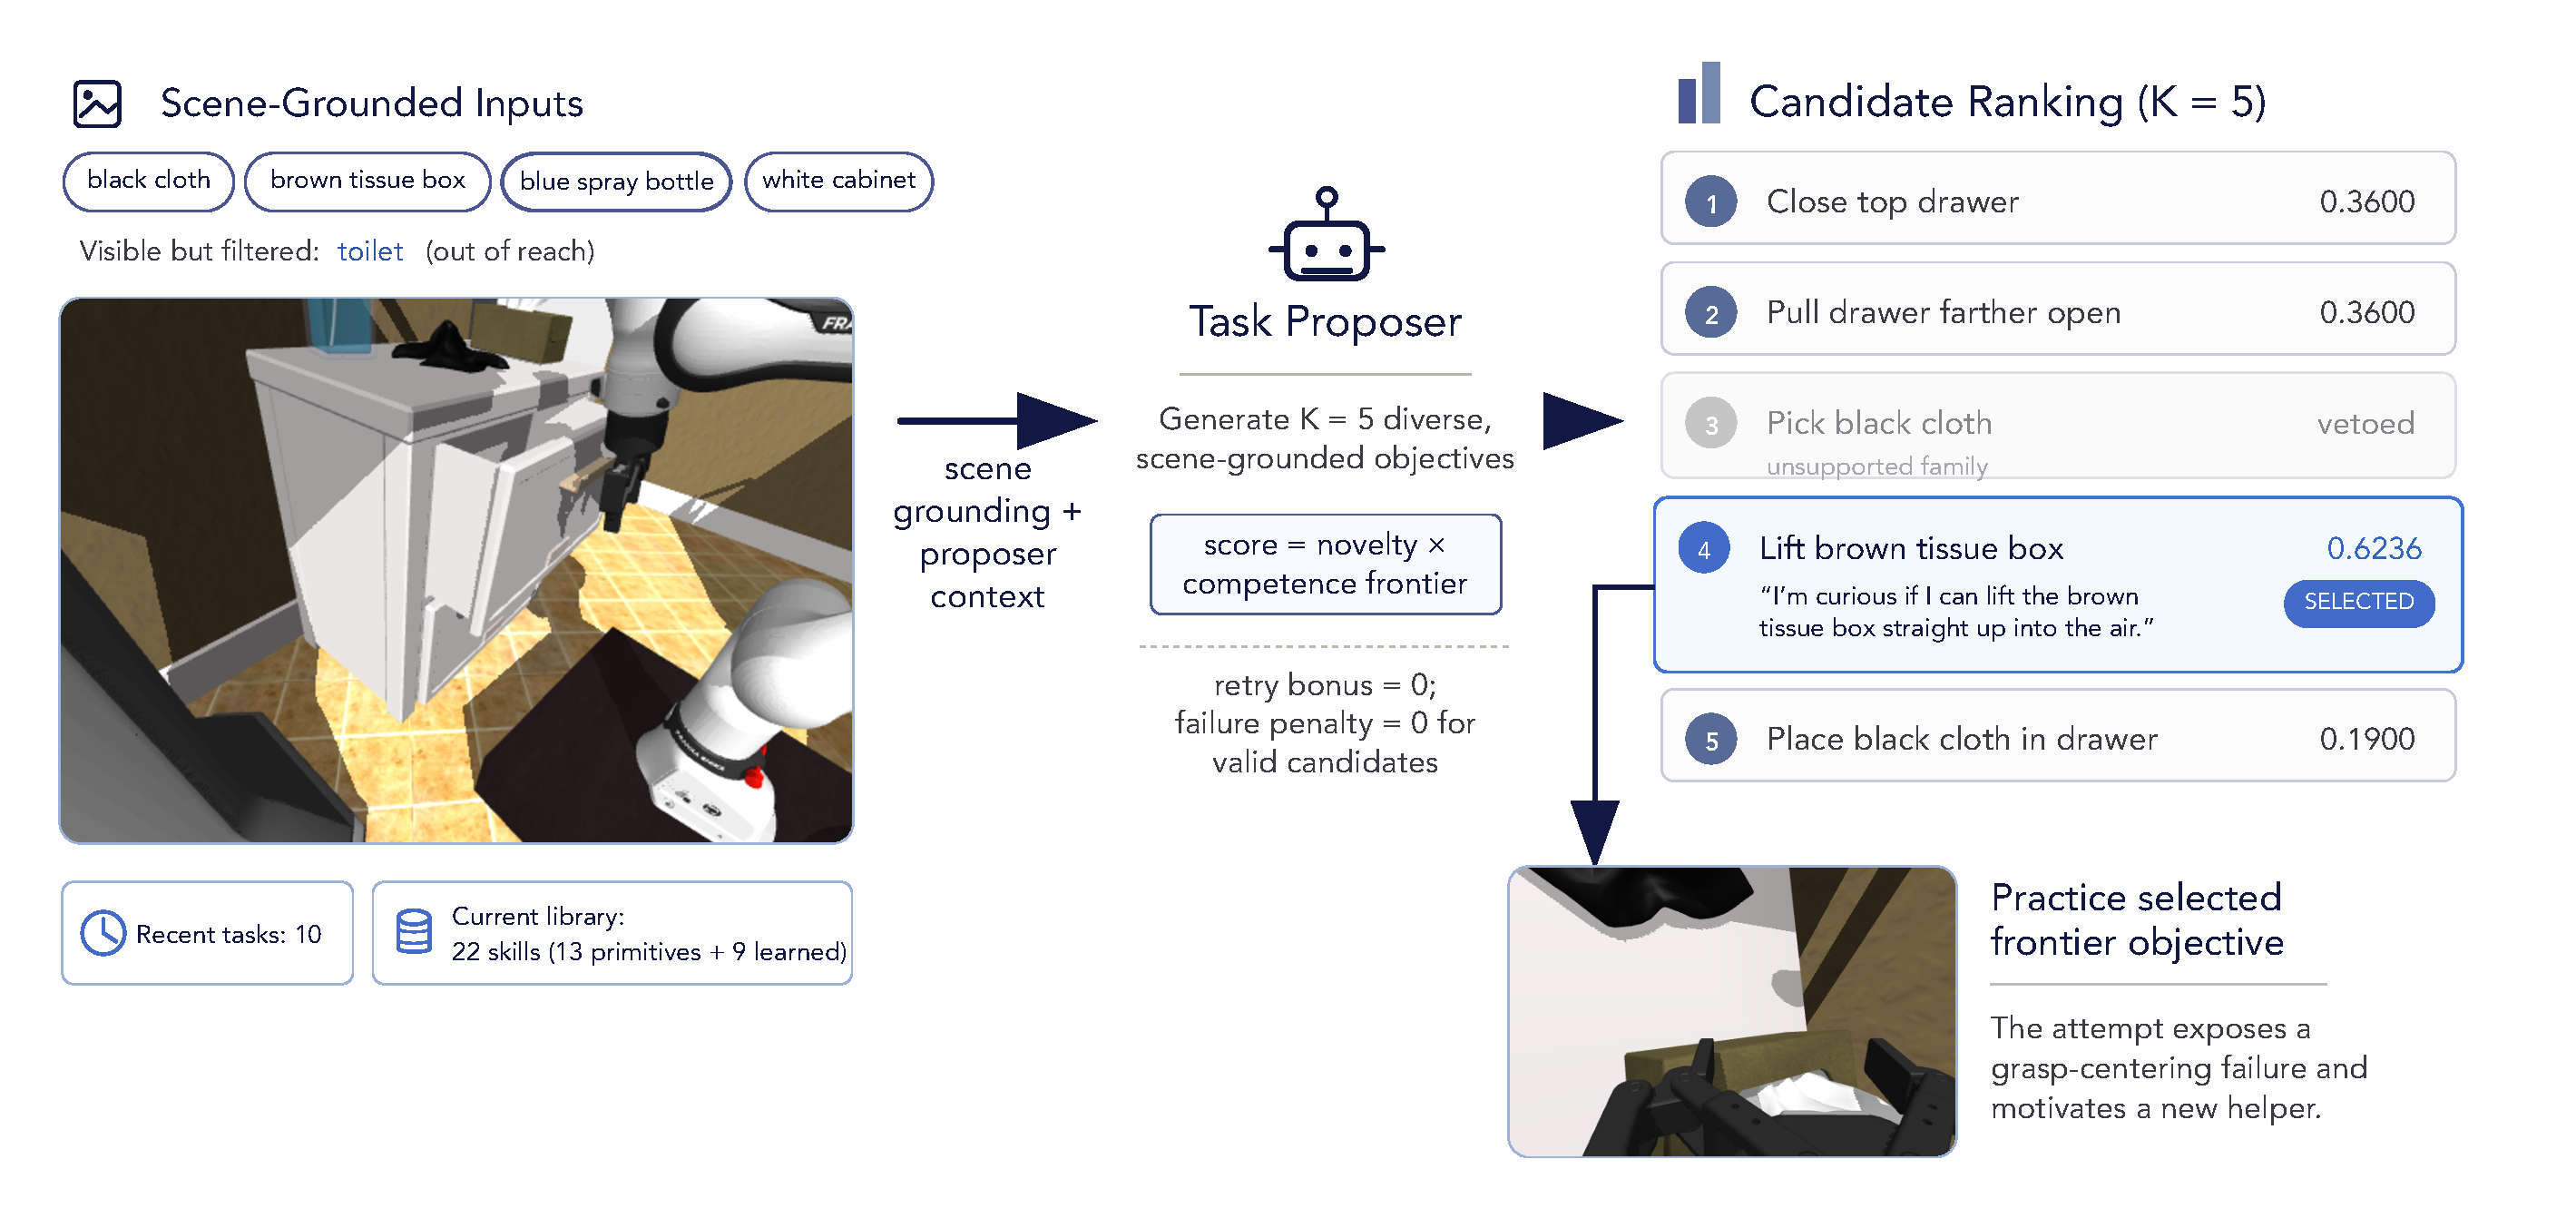
\includegraphics[width=\linewidth]{figs/appendix/task_proposal_ex.pdf}
\vspace{-1.5em}
\caption{
\textbf{Example trace of play-time task proposal.}
An example of the MolmoSpaces play-time task proposal process at iteration 15.
}
\label{fig:play_task_proposal}
\vspace{-1em}
\end{figure}

\textbf{Inputs to Task Proposer.}
The Task Proposer sees both low-level primitives and the learned skills
accumulated by earlier play. Its 13 primitives are grouped into
perception (\texttt{get\_observation}, \texttt{segment\_sam3\_text\_prompt},
\texttt{segment\_sam3\_point\_prompt}, \texttt{point\_prompt\_molmo}, and
\texttt{vlm\_verify}), grasp planning and control
(\texttt{plan\_grasp\_from\_point\_clouds}, \texttt{solve\_ik},
\texttt{move\_to\_joints}, \texttt{goto\_pose}, and
\texttt{goto\_home\_joint\_position}), and gripper control
(\texttt{open\_gripper}, \texttt{close\_gripper}, and
\texttt{select\_top\_down\_grasp}). Table~\ref{tab:proposal_skill_snapshot}
lists the nine learned skills by function name. The displayed success
rates are the raw metadata shown to the proposer; the analytical ranker uses
Wilson-bounded reliability instead.

\begin{table*}[t]
\centering
\scriptsize
\setlength{\tabcolsep}{4pt}
\caption{
\textbf{Learned-skill snapshot provided to the Task Proposer at
MolmoSpaces play iteration 15.}
The prompt additionally contains the 13 primitive function names listed in the
preceding paragraph. ``Raw rate'' is the success-rate metadata in the prompt, not the
Wilson-bounded value used for analytical selection.
}
\label{tab:proposal_skill_snapshot}
\vspace{1.5em}
\begin{tabular}{p{0.31\textwidth} p{0.42\textwidth} c c c}
\toprule
\textbf{Learned skill in prompt} & \textbf{Reusable capability} &
\textbf{Raw rate} & \textbf{Uses} & \textbf{Tier} \\
\midrule
\skill{localize\_object\_with\_molmo\_sam3} & Localize an object from agent-view Molmo prompting and SAM3 segmentation. & 0.3125 & 32 & Exp. \\
\skill{plan\_top\_down\_grasp\_at\_wrist} & Move the wrist camera over an object and plan a top-down grasp from segmented point clouds. & 0.2500 & 16 & Ver. \\
\skill{get\_axis\_aligned\_pull\_direction} & Compute an axis-aligned pull direction from the target toward the robot base. & 0.4286 & 7 & Ver. \\
\skill{select\_grasp\_for\_pulling} & Select a handle grasp whose approach opposes a requested pull direction. & 0.0000 & 0 & Exp. \\
\skill{execute\_top\_down\_grasp\_and\_lift} & Approach from above, close the gripper, and lift from a target 3D position. & 0.4167 & 12 & Ver. \\
\skill{push\_surface\_inward} & Push a surface inward to close a drawer or door. & 1.0000 & 2 & Exp. \\
\skill{execute\_grasp\_from\_transform} & Execute a grasp pose with a collision-avoidance height offset, then lift. & 0.2000 & 5 & Exp. \\
\skill{translate\_grasped\_object\_and\_release} & Translate a grasped object, release it, and retreat vertically. & 0.2000 & 5 & Exp. \\
\skill{push\_object\_closed} & Localize an open articulation, infer its outward direction, and push inward. & 1.0000 & 1 & Exp. \\
\bottomrule
\end{tabular}
\end{table*}

The proposer is also instructed to vary from the last ten attempts, avoid exact
verb-target duplicates, build one-variable-changed experiments from successes,
and simplify or change direction after failures. Table~\ref{tab:proposal_history}
transcribes the exact task-language field, success flag, and retry count inserted
into this prompt. Its diagnostic column condenses the accompanying
\texttt{failure\_reason} field while retaining the concrete failure mode and
suggested argument change.

\begin{table*}[t]
\centering
\scriptsize
\setlength{\tabcolsep}{4pt}

\caption{
\textbf{Recent objectives and outcomes supplied to the Task Proposer.}
The previous ten tasks and their successes are supplied to the Task Proposer. Relevant learned skills or failure diagnoses are listed as well.
}
\label{tab:proposal_history}
\vspace{1.5em}
{\renewcommand{\arraystretch}{1.1}
\begin{tabular}{c p{0.37\textwidth} c c p{0.42\textwidth}}
\toprule
& \textbf{Previous task language in prompt} & \textbf{Success} &
\textbf{Retries} & \textbf{Learned skill or failure diagnosis} \\
\midrule
1 & I wonder what happens if I lift the lever straight up into the air. & Yes & 0 & -- \\
2 & I want to see if I can push the top drawer all the way closed. & Yes & 0 & Learned \texttt{push\_surface\_inward}. \\
3 & Let's lift the brown sandal straight up. & Yes & 3 & -- \\
4 & I'm curious what happens when I lift the yellow button straight up. & Yes & 0 & -- \\
5 & I want to see what happens when I lift the toothpaste tube. & No & 4 & \texttt{grasp\_failure: argument\_level}. The $0.025$\,m grasp \texttt{z\_offset} left the fingers above the thin tube; the diagnosis suggests $0.0$ or $-0.01$\,m. \\
6 & Let's try to lift the blue clothes iron straight up and see what happens. & Yes & 0 & -- \\
7 & I wonder what happens if I lift the black videocassette straight up. & No & 4 & \texttt{collision: argument\_level}. Subtracting $0.035$\,m placed the grasp below the table; the diagnosis suggests subtracting $0.015$ or $0.02$\,m. \\
8 & I wonder if I can pull the walkie-talkie closer to me on the bed. & Yes & 0 & Learned two skills; \texttt{execute\_grasp\_from\_transform} and \texttt{translate\_grasped\_object\_and\_release}. \\
9 & I wonder if I can pull the metal ring closer to me across the table. & No & 4 & \texttt{grasp\_failure: rewrite\_needed}. The fingers missed or slipped from the knot; the diagnosis suggests targeting the center hole or subtracting $0.015$\,m from the grasp-pose height. \\
10 & I want to see if I can push the partially open drawer closed. & Yes & 0 & Learned \texttt{push\_object\_closed}. \\
\bottomrule
\end{tabular}
}
\end{table*}

\textbf{Why these candidates are proposed.}
Closing the top drawer is a nearby one-variable variation
of the two successful drawer-closing tasks and can reuse
\texttt{push\_object\_closed}. Pulling the drawer farther open probes the
opposite articulation direction while reusing the available pull-direction and
handle-grasp helpers. Picking up the cloth and placing it inside the open drawer
exercise two under-explored interactions on a visible object. Finally, lifting the
tissue box applies the verified top-down lift routine to a novel visible
object. This causal reading is an interpretation of the recorded prompt and
candidate rationales: the trace does not log token-level attribution inside the
proposer LLM.

\textbf{Why the tissue-box lift task is selected.}
The ranker uses
$s(\tau)=\mathcal{N}(\tau)\mathcal{F}(\tau)+w_BB_{\mathrm{retry}}(\tau)
-w_PP_{\mathrm{fail}}(\tau)$ for scoring tasks. Here, $\mathcal{F}$ is the competence-frontier learnability term. The analytical ranker computes
object-skill novelty and obtains $\mathcal{N}=1.0$ for every
candidate because each projected target-action pair is new. Surprise is used
only inside the retry-bank bonus path; this proposal turn has no surprise value, so $B_{\mathrm{retry}}=0$. None of the candidates
is sufficiently similar to a recent failed task to receive a failure penalty.

The remaining difference is therefore the competence frontier. For drawer closing and
opening, known primitive baselines
(\texttt{close\_gripper} and \texttt{open\_gripper}) and learned skills (\texttt{push\_object\_closed}) are used in competence calculation, yielding
$\bar{r}=0.9$ and $\mathcal{F}=4(0.9)(0.1)=0.36$. The cloth placement projects to \texttt{place\_in} family, for which the
library has no matching helper; the missing-skill default $\bar{r}=0.05$ gives
$\mathcal{F}=0.19$. The tissue-box lift projects to \texttt{lift} family, which
matches \texttt{execute\_top\_down\_grasp\_and\_lift}. That helper has five
successes in 12 uses: its raw prompt rate is $0.4167$, while its conservative
Wilson lower bound is $\bar{r}=0.1933$. Consequently,
$\mathcal{F}=4(0.1933)(1-0.1933)=0.6236$. The lift is neither already mastered
nor entirely unsupported, so it receives the highest Goldilocks score. After
selection, the tissue-box practice task remains unsuccessful after four
attempts and exposes a grasp-centering bottleneck, motivating the proposed
helper \texttt{adjust\_grasp\_to\_centroid}.

\begin{table*}[t]
\centering
\scriptsize
\setlength{\tabcolsep}{4pt}
\caption{
\textbf{Candidate-selection trace from MolmoSpaces play iteration 15.}
The Task Proposer generates five scene-grounded alternatives and the analytical
ranker selects a learnable frontier objective after bridge-compatibility
checks. A dash in the surprise column indicates that surprise
value is zero for this play-time proposer turn.
}
\label{tab:proposal_selection_example}
\vspace{1.5em}
\begin{tabular}{p{0.3\textwidth} l c c c c c c c p{0.05\textwidth}}
\toprule
\textbf{Candidate objective} & \textbf{Family} & $\mathcal{N}$ & $\bar{r}$ &
$\mathcal{F}$ & \textbf{Surp.} & $w_BB_{\mathrm{retry}}$ &
$w_PP_{\mathrm{fail}}$ & \textbf{Score} & \textbf{Result} \\
\midrule
Push the top drawer of the white cabinet all the way closed. & Close & 1.0000 & 0.9000 & 0.3600 & -- & 0.0000 & 0.0000 & 0.3600 & Valid \\
Pull the partially open drawer out even more. & Open & 1.0000 & 0.9000 & 0.3600 & -- & 0.0000 & 0.0000 & 0.3600 & Valid \\
Pick up the black cloth from the cabinet. & Pick & -- & -- & -- & -- & -- & -- & 0.0000 & Vetoed \\
Lift the brown tissue box straight up into the air. & Lift & 1.0000 & 0.1933 & 0.6236 & -- & 0.0000 & 0.0000 & 0.6236 & Selected \\
Put the black cloth inside the open drawer. & Place in & 1.0000 & 0.0500 & 0.1900 & -- & 0.0000 & 0.0000 & 0.1900 & Valid \\
\bottomrule
\end{tabular}
\end{table*}

\subsection{Details of \textsc{RATs} for Execution}
\label{sec:appendix_execution}

\textsc{RATs} executes each accepted task through a bounded
Write-Execute-Verify-Diagnose loop. The loop is designed to localize failures
to planning, code generation, or physical execution before the next retry.

\textbf{Planner.}
The Planner receives the task description, the initial scene observation,
retrieved lessons from failure memory, primitive APIs, and active learned
skills. Skills are ordered by reliability: verified skills are shown before
experimental skills, while deprecated skills are hidden by default. The Planner
outputs an ordered plan, annotates each step with relevant skills, and predicts
likely failure points for downstream inspection.

\textbf{Planner Verifier.}
Before code generation, the Planner Verifier checks whether the plan is grounded
in the initial observation. It looks for scene misperception, missing
preconditions, incorrect action ordering, and object-scope mismatch. If the
issue is correctable, the Planner revises the plan using the verifier's
feedback. This refinement repeats until the plan passes or reaches the
refinement budget.

\textbf{Policy Writer.}
The Policy Writer converts the verified plan into executable Python code. Its
prompt includes selected skill references, primitive API documentation,
retrieved failure lessons, and feedback from previous attempts. On retry, it
also receives per-step verification results and a summary of code segments that
already worked, encouraging local edits instead of rewriting the full policy.

\textbf{Quality Checker.}
Before execution, the Quality Checker statically screens the generated code. It
rejects syntax errors, unavailable API calls, unbounded loops, forbidden code
patterns, and malformed result reporting. This avoids spending robot
interaction budget on errors that can be detected from source code alone.

\textbf{Goal Verifier.}
After execution, the Goal Verifier determines task success. When a structured
predicate is available, success is evaluated from environment state. Otherwise,
the verifier uses a structured custom check or visual judgment. A policy crash
always counts as failure, even if the final visual state appears plausible.

\textbf{Per-Step Verifier.}
The Per-Step Verifier provides localized evidence for diagnosis. For each plan
step, it receives the step objective, corresponding code slice, critical runtime
values, and before/after visual evidence, including a short motion clip when
available. It returns a step-level verdict and explanation, distinguishing, for
example, a failed grasp from a successful grasp followed by an incorrect
placement.

\textbf{Failure Diagnoser.}
When a task fails, the Failure Diagnoser reads the execution trace, terminal
state, goal-verifier result, and per-step verdicts. It returns a failure
category, the first failed step, a concrete repair suggestion, and optional
routing flags. Code-local failures are routed back to the Policy Writer.
Plan-level failures trigger plan refinement. Persistent local physical
bottlenecks can spawn a SubAgent.

\textbf{SubAgent.}
The SubAgent practices a single failed sub-action, such as a grasp or
articulation, in the same reset state. It evaluates candidate scripts and
returns the first visually verified reusable helper routine. The winning
routine is inserted into the Policy Writer context for the current retry, so it
can be reused at the failed step. It is not automatically promoted into the
persistent skill library; promotion happens only after the routine contributes
to a successful end-to-end execution or is separately proposed and validated.
This keeps useful SubAgent discoveries available without polluting the library
with overfitted local fixes.

\subsection{Details of Skill Library and Failure Memory Updates}
\label{sec:appendix_skill_memory}

\textsc{RATs} maintains two persistent stores: the skill library $\mathcal{L}$
and the failure memory $\mathcal{M}$. Both are updated after each play attempt
and periodically curated to keep retrieval useful.

\textbf{Skill library.}
Each skill in $\mathcal{L}$ stores executable Python source code, a
description, preconditions, expected effects, dependencies, provenance, usage
counts, success counts, and a reliability tier. New code is parsed and
validated before insertion. The validation checks that the helper defines a
callable function, uses only available primitives or known dependencies, and
does not duplicate an existing skill. The library exposes a metadata-only view
for task proposal and a code-bearing view for planning and execution.

\textbf{Skill reliability.}
Skills follow a three-tier reliability lifecycle. A new skill starts as
\emph{experimental}. It is promoted to \emph{verified} after at least three
uses with empirical success rate at least $0.5$, and marked
\emph{deprecated} after at least ten uses with success rate at most $0.2$.
Verified skills can be demoted after sustained poor performance. Retrieval
prioritizes verified skills using Wilson-bounded reliability and hides
deprecated skills by default. At execution time, the runtime injects selected
skill definitions and their dependencies into the policy namespace, while
keeping active helpers available as a dependency-safety fallback.

\textbf{Skill extraction on success.}
After a successful end-to-end trajectory, the system extracts self-contained,
parameterized helper functions from the executed policy. The extracted helpers
capture reusable behavioral units rather than entire task scripts. They are
statically validated and inserted into $\mathcal{L}$ as experimental skills.
The successful trajectory also updates usage statistics for any learned skills
invoked during execution.

\textbf{Failure memory on failure.}
On failure, the system records the episode in $\mathcal{M}$. Each raw episode
stores the task, involved objects, failure category, failed plan step,
diagnostic explanation, attempted approach, and relevant code excerpt. Related
failures are distilled into compact lessons: when a condition occurs, avoid the
failed approach and use the suggested correction. The Planner retrieves lessons
by task and object overlap, allowing later attempts to benefit from prior
failures without replaying long traces in the prompt.

\textbf{Memory curation and skill proposal.}
Every $K$ play iterations, the Memory Curator merges, rewrites, or removes
redundant lessons and near-duplicate skills. When repeated failures reveal a
missing capability, the Skill Proposer drafts a candidate helper from
primitives and learned skills. Unlike skill extraction, which stores code that
has already succeeded, the Skill Proposer is anticipatory: the proposed helper
enters $\mathcal{L}$ as experimental and earns reliability only through later
use.

\subsection{Details of Evaluation With the Learned Skill Library}
\label{sec:appendix_test_time}


At test time, the learned library $\mathcal{L}$ is frozen and evaluated on
externally specified benchmark tasks. Task proposal and memory curation are disabled. We evaluate the learned library in two settings:
plug-and-play execution with a standard Code-as-Policy baseline, and full
\textsc{RATs} execution.


\paragraph{Plug-and-Play \textsc{CaP-Agent0} evaluation.}
In the plug-and-play setting, learned skills are loaded from the frozen library
and exposed to a standard single-agent Code-as-Policy baseline, \textsc{CaP-Agent0}.
Each selected skill's signature, description, and source code are added to the
baseline API context, and the function definitions are inserted into the
execution namespace. For large libraries, a lightweight selector can retrieve a
task-relevant subset before prompt construction. This setting omits the
\textsc{RATs} Planner, verification-driven retry loop, and failure-memory
retrieval, isolating the transfer value of the learned code library itself.

\paragraph{\textsc{RATs} evaluation.}
In the full \textsc{RATs} setting, the same frozen library is provided to the
Planner. The Planner receives primitive APIs and active learned skills,
prioritizes verified skills over experimental ones, and selects relevant skills
for individual plan steps. The Policy Writer then generates code conditioned on
these selected skills, while the runtime injects their executable definitions
and dependencies. Goal verification, per-step verification, diagnosis, and
bounded retry remain active. This setting measures the combined value of
play-time skill acquisition and the \textsc{RATs} execution loop on unseen
tasks.
